\documentclass[11pt]{article}

\usepackage{a4wide}
\usepackage[utf8]{inputenc}
\usepackage[russian]{babel}
\usepackage{graphicx}
\usepackage{amsmath}
\usepackage{amsthm}
\usepackage{amssymb}

\newtheorem{theorem}{Теорема}
\newtheorem{defenition}{Определение}
\newtheorem{proposition}{Утверждение}

\newcommand*{\hm}[1]{#1\nobreak\discretionary{}{\hbox{$\mathsurround=0pt #1$}}{}}
\newcommand\abs[1]{\left\lvert#1\right\rvert}
\newcommand{\scalar}[2]{\left<#1,#2\right>}
\newcommand{\norm}[1]{\left\lVert #1 \right\lVert}
\renewcommand{\d}[1]{\ensuremath{\operatorname{d}\!{#1}}}

\begin{document}
\thispagestyle{empty}

\begin{center}
\ \vspace{-3cm} \newline
\includegraphics[width=0.5\textwidth]{msu.eps}\\
{\scshape Московский государственный университет имени М.~В.~Ломоносова}\\
Факультет вычислительной математики и кибернетики\\
Кафедра системного анализа

\vfill

{\LARGE Отчёт по практикуму <<Оптимальное управление>>} \newline
%\vspace{1cm}
{\Huge\bfseries Задание 1: линейная задача быстродействия}
\end{center}

\vspace{1cm}
\begin{flushright}
\large
\textit{Студент 315 группы}\\
В.~С.~Терёшин\\
%\vspace{5mm}
%\textit{Руководитель практикума}\\
%к.ф.-м.н., доцент П.~П.~Петров
\end{flushright}

\vfill
\begin{center}
Москва, 2014
\end{center}
\pagebreak
\tableofcontents
\pagebreak
\section{Постановка задачи}
Задана линейная система обыкновенных дифференциальных уравнений:
\begin{gather}
\dot{x} = A(t)x + B(t)u, \; t \in [t_0, +\infty). \label{MainEquation} \\
t_1 - t_0 \longrightarrow \min \notag
\end{gather}
Здесь $x \in \mathbb{R}^2$, $A(t) \in \mathbb{R}^{2 \times 2}$, $B(t) \in \mathbb{R}^{2 \times 2}$, $u \in \mathbb{R}^2$. На значения управляющих параметров $u$ наложено ограничение: $u \in \mathcal{P}$. Пусть $\mathcal{X}_0$ --- начальное множество значений фазового вектора, $\mathcal{X}_1$ --- целевое множество значений фазового вектора. Необходимо решить задачу быстродействия, то есть найти минимальное время $T > 0$, за которое траектория системы, выпущенная в момент времени $t_0$ из некоторой точки $\mathcal{X}_0$, может попасть в некоторую точку множества $\mathcal{X}_1$.

$\mathcal{P}$ --- невырожденный эллипсоид с матрицей конфигурации $Q = Q' > 0$ и центром в точке $p$,
\begin{gather}
\mathcal{X}_0 = \left\{ \left( x_1, x_2 \right)' : \, \left( x_1 - \alpha_1 \right)^2 + \left( x_2 - \alpha_2 \right)^4 \leqslant 1\right\}, \notag \\
\mathcal{X}_1 = \left\{ \left( x_1, x_2 \right)' : \, x_1 x_2 \geqslant 1, \, x_1 \geqslant 0, \, x_1 + x_2 \leqslant a \right\}, \; a > 0. \notag
\end{gather}

Необходимо написать в среде \texttt{Matlab} программу с пользовательским интерфейсом, которая по заданным параметрам $A(\cdot)$, $B(\cdot)$, $t_0$, $Q$, $p$, $a$, $\alpha_1$, $\alpha_2$ определяет, разрешима ли задача быстродействия. Если задача разрешима, то программа должна (приближённо) найти значение $T$, построить графики компонент оптимального управления, компонент оптимальной траектории, сопряжённых переменных. Программа должна рассчитывать погрешность выполнения условий трансверсальности для найденной <<оптимальной>> траектории. Программа должна давать пользователю возможность постепенно улучшать результаты расчётов за счёт изменения параметров численного метода и анализа результатов.

Дополнительно будем считать, что все компоненты матриц $A(t)$ и $B(t)$ непрерывно зависят от времени. Управление будем искать в классе кусочно-непрерывных функций. В этом случае компоненты траектории будут непрерывными и кусочно-гладкими по времени.
\section{Теория}
\subsection{Принцип максимума Понтрягина}
Пусть дана задача быстродействия:
\begin{gather}
\dot{x} = A(t)x + B(t)u, \notag \\
x^0 \in \mathcal{X}_0, \notag \\
x^1 \in \mathcal{X}_1, \notag \\
u(t) \in \mathcal{P}, \notag \\
t_1 - t_0 \longrightarrow \min. \notag
\end{gather}
со сделанными выше предположениями относительно $A(t)$, $B(t)$, $u(t)$. Тогда справедлива следующая теорема:
\begin{theorem} \label{PMP}
Пусть $\left( x^*(t), u^*(t) \right)$ - оптимальная пара, $u^*(t)$ переводит фазовую точку из положения $x^0 \in \mathcal{X}_0$ в положение $x^1 \in \mathcal{X}_1$ за время $T$. Тогда существует непрерывная вектор-функция $\psi(t)$, нигде не обращающаяся в нуль и удовлетворяющая следующим условиям:
\begin{gather}
\dot{\psi} = -A^T(t)\psi, \label{PMP2} \\
\scalar{B^T(t)\psi(t)}{u^*(t)} = \rho(B^T(t)\psi(t) \mid \mathcal{P}), \label{PMP3} \\
\scalar{\psi(t_0)}{x^0} = \rho(\psi(t_0) \mid \mathcal{X}_0), \label{PMP4} \\
\scalar{-\psi(t_1)}{x^1} = \rho(-\psi(t_1) \mid \mathcal{X}_1). \label{PMP5}
\end{gather}
Функцию $\psi(t)$ называют сопряжённой функцией.
\end{theorem}
\subsection{Вычисление опорных функций}
\begin{defenition}
Опорной функцией множества $A \subset \mathbb{R}^n$ называется $\rho(l \mid A) = \sup\limits_{x \in A} \scalar{x}{l}$, $l \in \mathbb{R}^n$.
\end{defenition}
\begin{proposition}
Пусть $A \subset \mathbb{R}^n$ --- ограниченное замкнутое множество. Тогда $\sup\limits_{x \in A} \scalar{x}{l}$ достигается, причём на границе $A$.
\end{proposition}
\subsubsection{Опорная функция $\mathcal{P}$}
$\mathcal{P}$ --- эллипс с матрицей конфигурации $Q > 0$ и центром в $p$. Его уравнение:
$$
\scalar{x - p}{Q^{-1}(x - p)} \leqslant 1.
$$
Вектор, соответствующий опорной функции для аргумента $\left( x_1^0, x_2^0\right)$, будем искать на границе $\mathcal{P}$, то есть там, где
$$
\scalar{x - p}{Q^{-1}(x - p)} = 1.
$$
Раскроем скалярное произведение, обозначив $Q^{-1}$ за $A$:
\begin{gather}
\scalar{x - p}{A(x - p)} - 1 = 0 \notag \\
(x_1 - p_1) (A_{11}(x_1 - p_1) + A_{12}(x_2 - p_2) + (x_2 - p_2) (A_{21}(x_1 - p_1) + A_{22}(x_2 - p_2)) - 1 = \notag \\
= A_{11} x_1^2 + A_{22} x_2^2 + (A_{12} + A_{21}) x_1 x_2 + \notag \\
+ (-2 A_{11} p_1 - (A_{12} + A_{21}) p_2) x_1 + (-2 A_{22} p_2 - (A_{12} + A_{21}) p_1) x_2 + \notag \\
+ (A_{11} p_1^2 + (A_{12} + A_{21}) p_1 p_2 + A_{22} p_2^2 - 1) = 0. \notag
\end{gather}
Обозначим коэффициеты перед $x_1^2$, $x_2^2$, $x_1 x_2$, $x_1$, $x_2$ и свободный член за $a$, $b$, $c$, $d$, $e$ и $f$ соответственно:
$$
a x_1^2 + b x_2^2 + c x_1 x_2 + d x_1 + e x_2 + f = 0.
$$
Воспользуемся методом Лагранжа:
\begin{gather}
L = x_1^0 x_1 + x_2^0 x_2 + \lambda \left( a x_1^2 + b x_2^2 + c x_1 x_2 + d x_1 + e x_2 + f \right), \notag \\
\frac{\d{L}}{\d{x_1}} = x_1^0 + 2\lambda a x_1 + \lambda c x_2 + \lambda d = 0, \notag \\
\frac{\d{L}}{\d{x_2}} = x_2^0 + 2\lambda b x_2 + \lambda c x_1 + \lambda e = 0, \notag \\
\frac{\d{L}}{\d{\lambda}} = a x_1^2 + b x_2^2 + c x_1 x_2 + d x_1 + e x_2 + f = 0. \notag
\end{gather}

Решим данную систему с помощью символьных вычислений среды \texttt{Matlab}. Получим два точных решения:
\begin{gather}
x_1 =
\frac{
	ce - 2bd \pm
	K\left(
		2bx_1^0 - cx_2^0
	\right)
}
{
    4ab - c^2
}
, \; \;
x_2 =
\frac{
	cd - 2ae \pm
	K\left(
		2ax_2^0 - cx_1^0
	\right)
}
{
    4ab - c^2
}
, \label{SF_P}
\end{gather}
где
$$
K =	\sqrt{\frac{fc^2 + bd^2 + ae^2 - cde - 4abf}
		{
			b
			\left(
				x_1^0
			\right)
			^2 - cx_1^0x_2^0 + a
			\left(
				x_2^0
			\right)
			^2
		}}.
$$

Одно из них соответствует минимуму скалярного произведения, а другое --- максимуму. Выберем то, которое соответствует максимуму --- это и будет решением данной задачи.
\subsubsection{Опорная функция $\mathcal{X}_0$}
Граница $\mathcal{X}_0$ описывается уравнением:
$$
\left( x_1 - \alpha_1 \right)^2 + \left( x_2 - \alpha_2 \right)^4 - 1 = 0.
$$
Для нахождения вектора $\left(x_1, x_2 \right)$, на котором достигается максимум скалярного произведения на $\left(x_1^0, x_2^0 \right)$, воспользуемся методом Лагранжа:
\begin{gather}
L = x_1^0 x_1 + x_2^0 x_2 + \lambda \left( \left( x_1 - \alpha_1 \right)^2 + \left( x_2 - \alpha_2 \right)^4 - 1 \right), \notag \\
\frac{\d{L}}{\d{x_1}} = x_1^0 + 2\lambda = 0, \notag \\
\frac{\d{L}}{\d{x_2}} = x_2^0 + 4\lambda\left(x_2 - \alpha_2\right)^3 = 0, \notag \\
\frac{\d{L}}{\d{\lambda}} = \left( x_1 - \alpha_1 \right)^2 + \left( x_2 - \alpha_2 \right)^4 - 1 = 0. \notag
\end{gather}
Выразим из первых двух уравнений $x_1$ и $x_2$:
\begin{gather}
x_1 = \frac{2\lambda\alpha_1 - x_1^0}{2\lambda}, \; x_2 = \sqrt[3]{\frac{-x_2^0}{4\lambda}} + \alpha_2. \label{SF_X0}
\end{gather}
Подставив в третье уравнение получим:
\begin{gather}
\left( \frac{2\lambda\alpha_1 - x_1^0}{2\lambda} - \alpha_1 \right)^2 + \left( \sqrt[3]{\frac{-x_2^0}{4\lambda}} \right)^4 - 1 = 0 \notag \\
\left( \frac{x_1^0}{2\lambda} \right)^2 + \left( \sqrt[3]{\frac{-x_2^0}{4\lambda}} \right)^4 - 1 = 0. \notag
\end{gather}
Заметим, что левая часть данного уравнения имеет предел равный $+\infty$ при $\lambda \longrightarrow 0$ и убывает при $\lambda > 0$, при этом очевидно, что решение существует.

Решим данное уравнение численно, воспользовавшись функцией \texttt{fzero} среды \texttt{Matlab} с начальным значением $\lambda = 1$ (это можно сделать в силу монотонного убывания левой части при $\lambda > 0$). Получим некоторое значение $\lambda$ и сооответствующие значения $x_1$, $x_2$. Однако это значение может быть не максимумом, а минимумом скалярного произведения. В силу центральной симметричности $\mathcal{X}_1$ относительно точки $\left( \alpha_1, \alpha_2 \right)$ необходимо также проверить точку $\left( 2\alpha_1 - x_1, 2\alpha_2 - x_2 \right)$. Посчитав скалярные произведения, выберем соответствующий максимизирующий вектор --- он и будет искомым.
\subsubsection{Опорная функция $\mathcal{X}_1$}
Граница $\mathcal{X}_1$ описывается системой уравнений:
$$
\left\{
\begin{aligned}
a - \frac{\sqrt{a^2 - 4}}{2} \leqslant x_1 \leqslant a + \frac{\sqrt{a^2 - 4}}{2} \\
\left[
\begin{aligned}
x_1 x_2 = 1 \\
x_1 + x_2 = a
\end{aligned}
\right. \\
\end{aligned}
\right.,
$$
что представляет из себя лунку в декартовых координатах.

Несложно видеть, что в зависимости от направления данного вектора $\left(x_1^0, x_2^0 \right)$ максимизирующий вектор $\left(x_1, x_2 \right)$ будет попадать либо в углы лунки, либо на её часть, описываемую уравнением $x_1 x_2 = 1$, либо на часть, соответствующую $x_1 + x_2 = a$. Возможные направления $\left(x_1^0, x_2^0 \right)$ разделим на зоны, определяемые нормалями к лунке.

Обозначим за $l = a - \tfrac{\sqrt{a^2 - 4}}{2}$ и $r = a + \tfrac{\sqrt{a^2 - 4}}{2}$ - координаты левого и правого угла лунки соответственно.

Пусть $t$ - тангенс угла наклона касательной к некоторой кривой на плоскости, задаваемой дифференцируемой выпуклой функцией. Тогда нормаль к этой кривой в этой точке --- это $\left( t, -1 \right)$.

Тогда все возможные направления $x^0 = \left(x_1^0, x_2^0 \right)$ разбиваются на:
\begin{enumerate}
\item
$x^0$ лежит между $\left( -\tfrac{1}{r^2}, -1 \right)$ и $\left( -\tfrac{1}{l^2}, -1 \right)$.
В этом случае максимизирующий вектор лежит на дуге, соответствующей $x_1 x_2 = 1$. Найдём максимизирующий вектор методом Лагранжа:
\begin{gather}
L = x_1^0 x_1 + x_2^0 x_2 + \lambda \left( x_1 x_2 - 1 \right), \notag \\
\frac{\d{L}}{\d{x_1}} = x_1^0 + \lambda x_2 = 0, \notag \\
\frac{\d{L}}{\d{x_2}} = x_2^0 + \lambda x_1 = 0, \notag \\
\frac{\d{L}}{\d{\lambda}} = x_1 x_2 - 1 = 0. \notag
\end{gather}
Решив эту систему, получим:
$$
\lambda = \pm \sqrt{x_1^0 x_2^0}, \; x_1 = \mp \sqrt{\frac{x_1^0}{x_2^0}}, \; x_2 = \mp \sqrt{\frac{x_2^0}{x_1^0}}.
$$
Осталось лишь выбрать ту пару $\left( x_1, x_2 \right)$, которая обеспечивает максимум скалярного произведения.
\item
$x^0$ лежит между $\left( -\tfrac{1}{l^2}, -1 \right)$ и $\left( 1, 1 \right)$ --- нормаль к $x_1 + x_2 = a$. В этом случае, очевидно, ответом является вектор $\left( l, \tfrac{1}{l} \right)$.
\item
$x^0$ лежит между $\left( 1, 1 \right)$ и $\left( -\tfrac{1}{r^2}, -1 \right)$. Аналогично предыдущему пункту ответом является вектор $\left( r, \tfrac{1}{r} \right)$.
\item
Если $x^0$ сонаправлен одному из векторов-границ, разделяющих направления, то можно считать, что он попал в любую из соответствующих частей разбиения.
\end{enumerate}
Таким образом, опорная функция $\mathcal{X}_1$ равна:
$$
\rho \left(x^0 \mid \mathcal{X}_1 \right) =
\begin{cases}
\abs{\scalar{\left( \sqrt{\frac{x_1^0}{x_2^0}}, \sqrt{\frac{x_2^0}{x_1^0}} \right)}{\left( x_1^0, x_2^0 \right)}}, & (1) \\
\scalar{\left( a - \frac{\sqrt{a^2 - 4}}{2}, \frac{2}{2a - \sqrt{a^2 - 4}} \right)}{\left( x_1^0, x_2^0 \right)}, & (2) \\
\scalar{\left( a + \frac{\sqrt{a^2 - 4}}{2}, \frac{2}{2a + \sqrt{a^2 - 4}} \right)}{\left( x_1^0, x_2^0 \right)}, & (3)
\end{cases}
$$
Принадлежность вектора $x^0$ к той или иной части разбиения будем определять с помощью псевдоскалярного произведения.
\section{Реализация}
\subsection{Основной алгоритм}
Рассмотрим принцип максимума Понтрягина для нашей задачи (теорема \ref{PMP}). Легко видеть, что, если функция $\psi(t)$ удовлетворяет всем условиям теоремы, то $m\psi(t)$ также будет им удовлетворять при любом $m > 0$. Значит, не ограничивая общности, можно считать, что $\norm{\psi(t_0)} = 1$.

Далее, пусть у нас есть $\psi(t) \neq 0$ $\forall t \geqslant t_0$ --- сопряжённая функция для оптимальной пары. Тогда, если $B^T(t)\psi(t) \neq 0$, то из условия \eqref{PMP3} однозначно определяется $u^*(t)$ соответствующее $\psi(t)$. $\psi(t) \neq 0$, а значит $x^*(t_0)$ также однозначно определяется по $\psi(t_0)$, а следовательно и вся траектория $x^*(t_0)$, как решение задачи Коши:
\begin{gather}
\dot{x} = A(t)x(t) + B(t)u(t),
x(t_0) = f(\psi(t_0)).
\end{gather}
Таким образом, если бы нам была известна сопряжённая функция, то по ней мы могли бы восстановить и оптимальную пару. С другой стороны, по теореме \ref{PMP}, если оптимальное решение существует, то сопряжённая функция удовлетворяет дифференциальному уравнению \eqref{PMP2}. Так же, как было сказано выше, можно считать, что $\norm{\psi(t_0)} = 1$. Из этого следует, что все возможные $\psi(t_0)$, а значит и $\psi(t) \forall t$ можно описать одним параметром. Ещё один параметр - это время прибытия фазовой точки во множество $\mathcal{X}_1$. Итак, мы имеем два параметра и неиспользованное второе условия трансверсальности \eqref{PMP5}, которое даёт два соотношения на параметры. Подобрав параметры, мы могли бы выделить класс управлений, подозрительных на оптимальность.

При решении задачи численно мы будем строить сетку на полуинтервали $\left[ 0, 2\pi \right]$: $0 = \phi_0 < \phi_1 < \dotsb < \phi_n < 2\pi$ и для каждого $\phi_i$ численно решать систему уравнений:
\begin{gather}
\dot{\psi} = -A^T\psi, \notag \\
\psi_1(t_0) = \cos(\phi_i), \notag \\
\psi_2(t_0) = \sin(\phi_i), \notag \\
u(t) = f_1(\psi(t)), \notag \\
\dot{x} = A(t)x(t) + B(t)u(t), \notag \\
x(t_0) = f_2(\psi(t)). \notag
\end{gather}
(здесь функция $f_1$ определяятся соотношениями \eqref{PMP3} и \eqref{SF_P}, а $f_2$ --- соотношениями \eqref{PMP4} и \eqref{SF_X0}) начиная с момента $t_0$ и до некоторого фиксированного $T_1$ или же до достижения фазовой переменной множества $\mathcal{X}_1$. После чего будем выбирать среди всех дошедших до $\mathcal{X}_1$ фазовых траекторий ту, которая сделала это за наименьшее время. Это наименьшее время и будет приближённым решением задачи.

Для решения системы дифференциальных уравнений воспользуемся стандартной функцией \texttt{Matlab} \texttt{ode45}, которая представляет из себя реализацию алгоритма Дормана--~Принса --- метод Рунге--~Кутты четвёртого--пятого порядка, автоматически подбирающего шаг так, чтобы локальные абсолютная и относительная погрешности были не больше некоторых напрерёд заданных чисел.

Проверка на то, пересекла ли траектория целевое множество $\mathcal{X}_1$ происходит на каждом шаге интегрирования с некоторой задаваемой пользователем погрешностью.
\subsection{Особый режим}
В случае $B^T(t)\psi(t) = 0$ воспользоваться принципом максимума Понтрягина для однозначного определения управления не получится. Поэтому изменим собственные значения (а значит и собственные векторы) матрицы $B$ на $\varepsilon$, задаваемый пользователем. Измененить собственные значения матрицы на $\varepsilon$ можно прибавив этот $\varepsilon$ к диагональным элементам матрицы.
\section{Техническая реализация и графический интерфейс пользователя}
Задание системы и управление решением осуществляется с помощью графического интерфейса пользователя, с помощью которого он может задать матрицы $A$, $B$, $Q$, точку $p$, параметры $a$, $\alpha_1$, $\alpha_2$ и начальное время $t_0$. Также пользователь задаёт максимальное время в системе \texttt{Tmax}, количество точек начальных условий на $\psi$ \texttt{Npoints} и шаг интегрирования траектории \texttt{time\_step}. Кроме того, возможно изменение погрешностей, используемых при решении:
\begin{enumerate}
\item
\texttt{touching\_X1} --- погрешность при определении попадания точки в конечное множество $\mathcal{X}_1$.
\item
\texttt{specific\_mode} --- погрешность при определении наличия особого режима ($\abs{B^T(t)\psi(t)} \hm< \texttt{specific\_mode}$).
\item
\texttt{zero\_in\_imag\_testing} --- допустимый модуль мнимой части числа, при которой оно считается вещественным.
\item
\texttt{rel\_tol}, \texttt{abs\_tol1,2} --- относительная и абсолютная погрешности, используемые в \texttt{ode45}.
\end{enumerate}

При успешном решении заданной задачи пользователю выдаётся наименьшее время, за которое возможно перевести систему из начального состояния в конечное при данных ограничениях, и погрешности выполнения условия трансверсальности в конечной точке траектории: абсолютную погрешность, равную $\abs{\scalar{-\psi(t_1)}{x^1} - \rho(-\psi(t_1) \mid \mathcal{X}_1)}$, и косинус угла между посчитанным вектором $\psi(t_1)$ (выделен на графике красным) и требуемым теорией (выделен зелёным). Также пользователю предлагается уточнить решение задачи: уменьшить промежуток начальных условий на $\psi$ в три раза вблизи найденного наилучшего решения. При клике на любом графике открывается его увеличенная копия.

В противном случае пользователю сообщается об отсутствии решения задачи при данных ограничениях и некоторые советы.
\section{Примеры работы}
\subsection{Пример 1}
$$
A = \left[
\begin{matrix}
\sin t & 0 \\
1 & \cos t
\end{matrix}
\right], \;
B = \left[
\begin{matrix}
\sin^2 t & \sin t^2\\
1 & 2
\end{matrix}
\right], \;
Q = \left[
\begin{matrix}
3 & 4 \\
4 & 6
\end{matrix}
\right], \;
t_0 = 0, \; p = \left( 1, -1 \right), \; a = 3, \; \alpha_1 = 2, \; \alpha_2 = 5.
$$
Количество начальных условий для $\psi$ возьмём равным 60. Результат работы --- оптимальное время 0.69, косинус между требуемым $\psi(t_1)$ в конечный момент и полученным равен 0.9807.

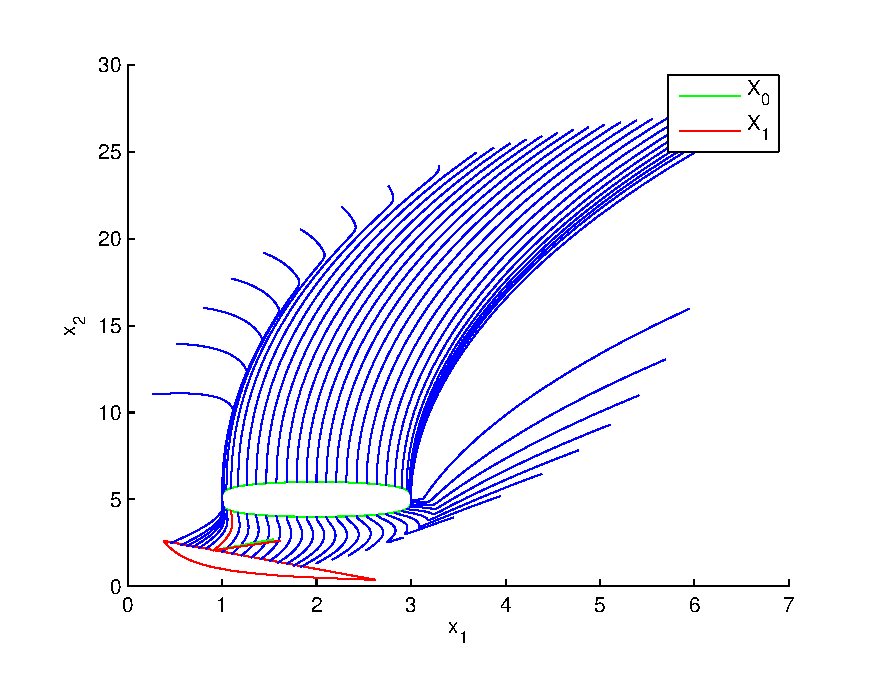
\includegraphics[scale=1]{pics/pic1_x.eps}

После первого уточнения получим оптимальное время 0.69 и косинус 0.9886:

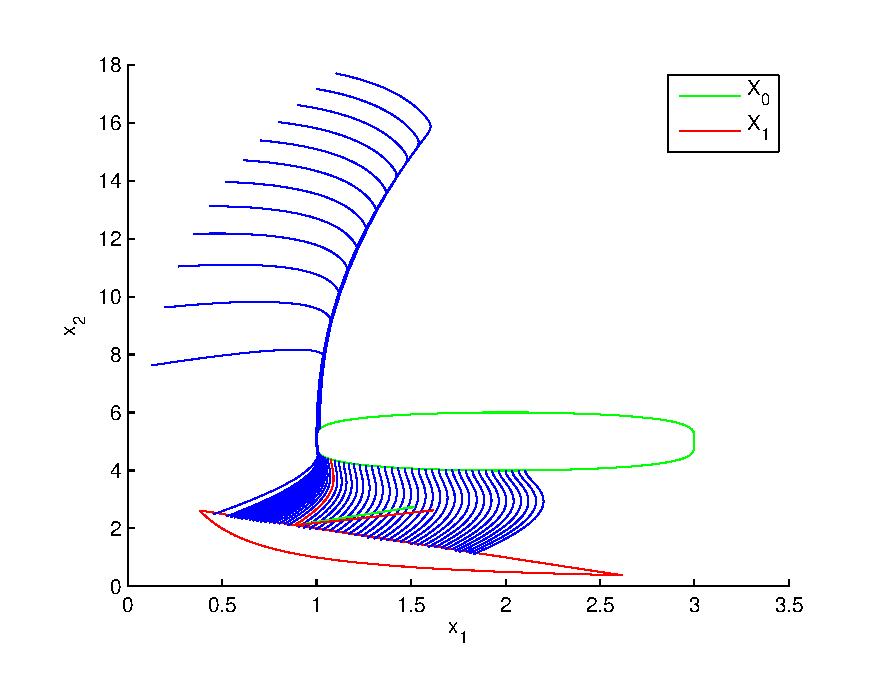
\includegraphics[scale=1]{pics/pic1_x_clar1.eps}

После второго уточнения получим оптимальное время 0.68997 и косинус 0.9913:

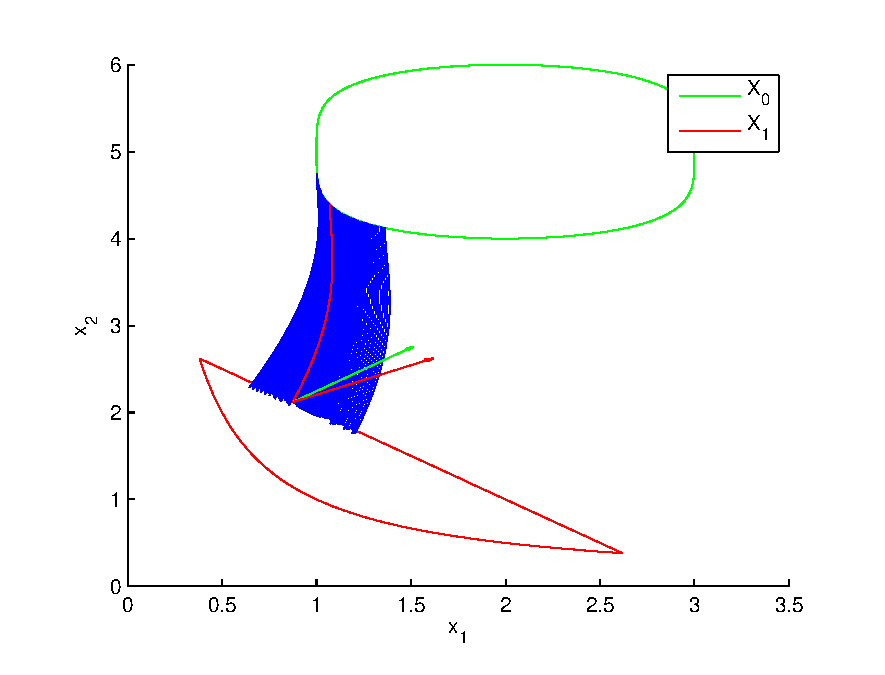
\includegraphics[scale=1]{pics/pic1_x_clar2.eps}

Остальные графики приведены для решения без уточнения:

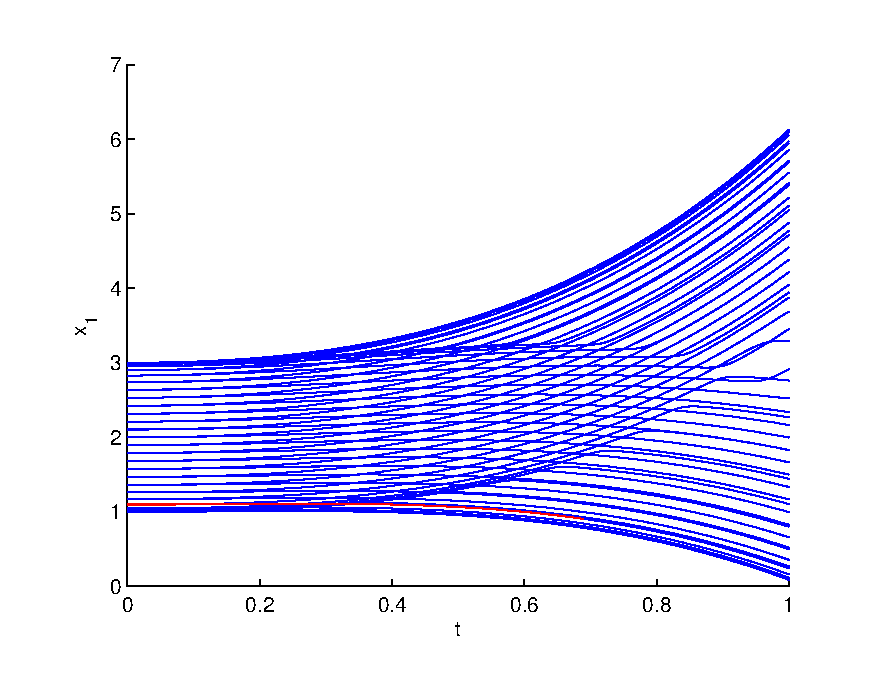
\includegraphics[scale=0.6]{pics/pic1_x1.eps}
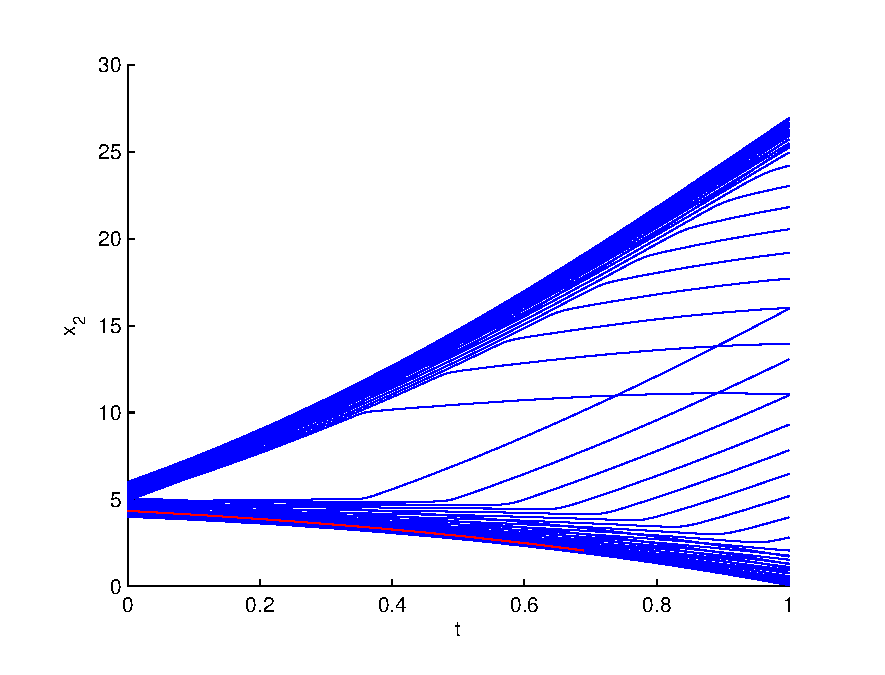
\includegraphics[scale=0.6]{pics/pic1_x2.eps}

\includegraphics[scale=0.6]{pics/pic1_u1.eps}
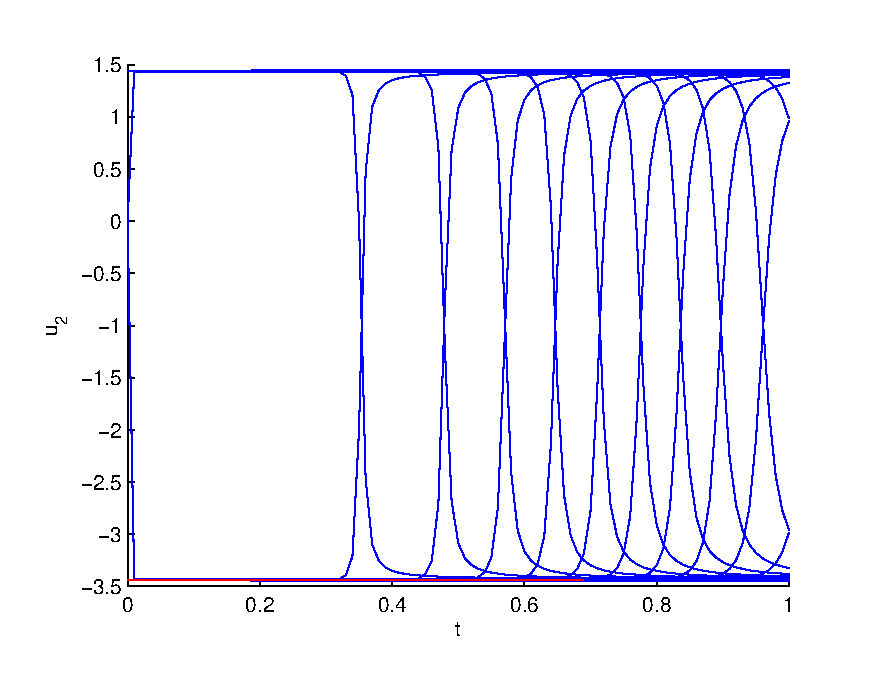
\includegraphics[scale=0.6]{pics/pic1_u2.eps}

\includegraphics[scale=0.6]{pics/pic1_phi1.eps}
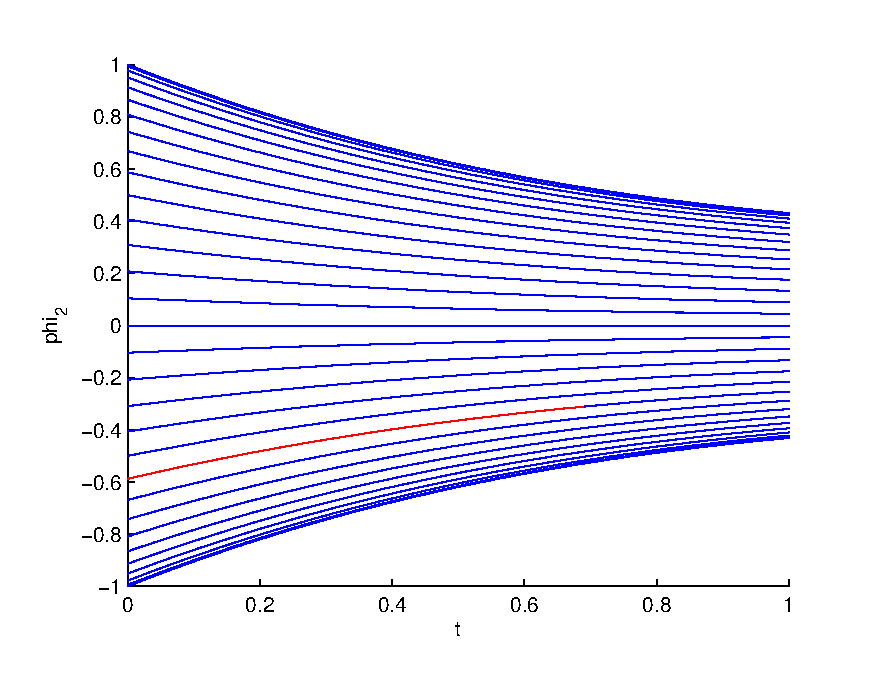
\includegraphics[scale=0.6]{pics/pic1_phi2.eps}

\includegraphics[scale=0.6]{pics/pic1_u.eps}
\subsection{Пример 2}
$$
A = \left[
\begin{matrix}
1 & 4 \\
-1 & -3
\end{matrix}
\right], \;
B = \left[
\begin{matrix}
-1 & 0 \\
2 & -2
\end{matrix}
\right], \;
Q = \left[
\begin{matrix}
3 & 4 \\
4 & 6
\end{matrix}
\right], \;
t_0 = 0, \; p = \left( 1, -1 \right), \; a = 3, \; \alpha_1 = -2, \; \alpha_2 = 2.
$$
Количество начальных условий для $\psi$ возьмём равным 60. Результат работы --- оптимальное время 0.13, косинус между требуемым вектором $\psi(t_1)$ и полученным равен 0.99.

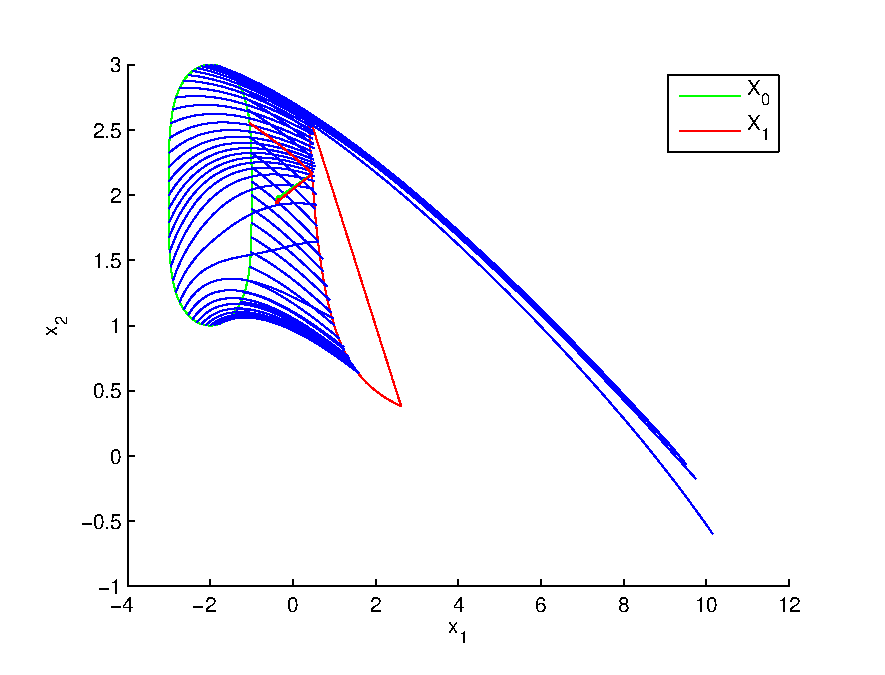
\includegraphics[scale=0.9]{pics/pic2_x.eps}

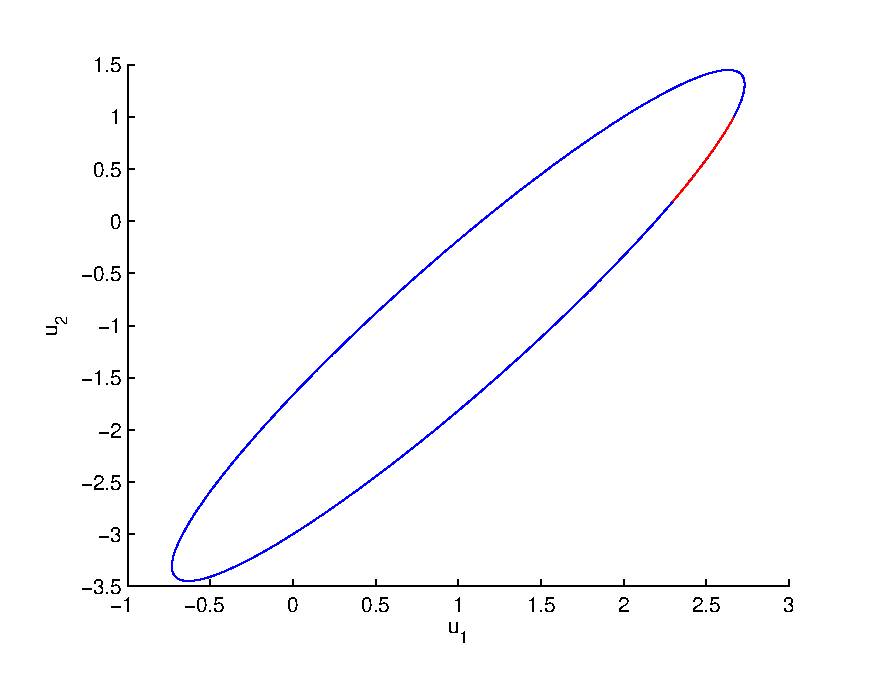
\includegraphics[scale=0.9]{pics/pic2_u.eps}

После первого уточнения получим время, равное 0.13 и косинус, равный 0.9951:

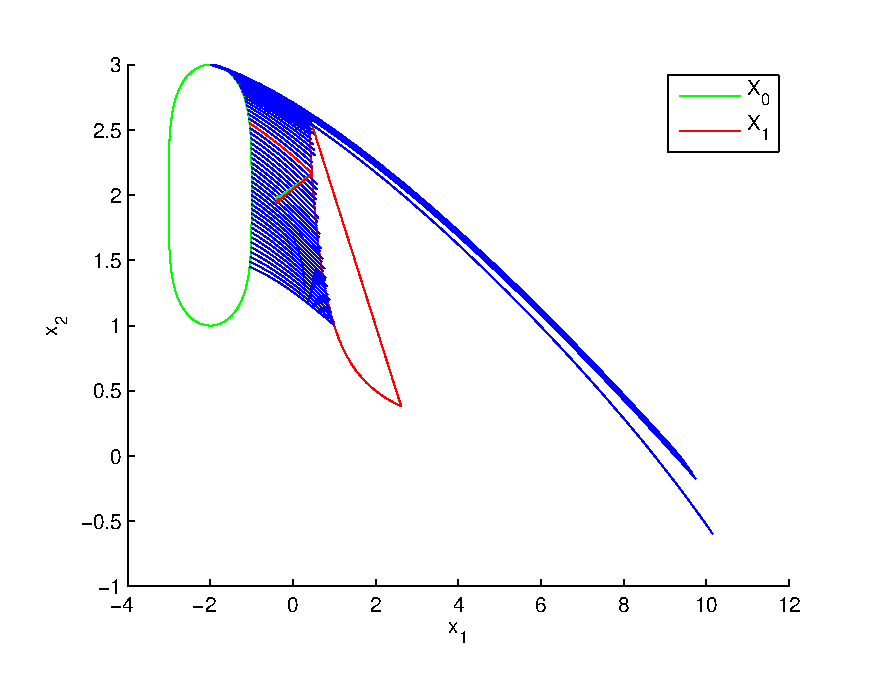
\includegraphics[scale=0.9]{pics/pic2_x_clar.eps}

\subsection{Пример отсутствия непрерывности времени по конечному множеству}
Рассмотрим систему:
$$
A = \left[
\begin{matrix}
\sin t & 0 \\
0 & -\cos t
\end{matrix}
\right], \;
B = \left[
\begin{matrix}
0.1 & 0 \\
0 & 0.1
\end{matrix}
\right], \;
Q = \left[
\begin{matrix}
3 & 4 \\
4 & 6
\end{matrix}
\right], \;
t_0 = 0, \; p = \left( 1, -1 \right), \; a = 7.11, \; \alpha_1 = 5, \; \alpha_2 = 5.
$$
Фазовые трактории выглядят следующим образом:

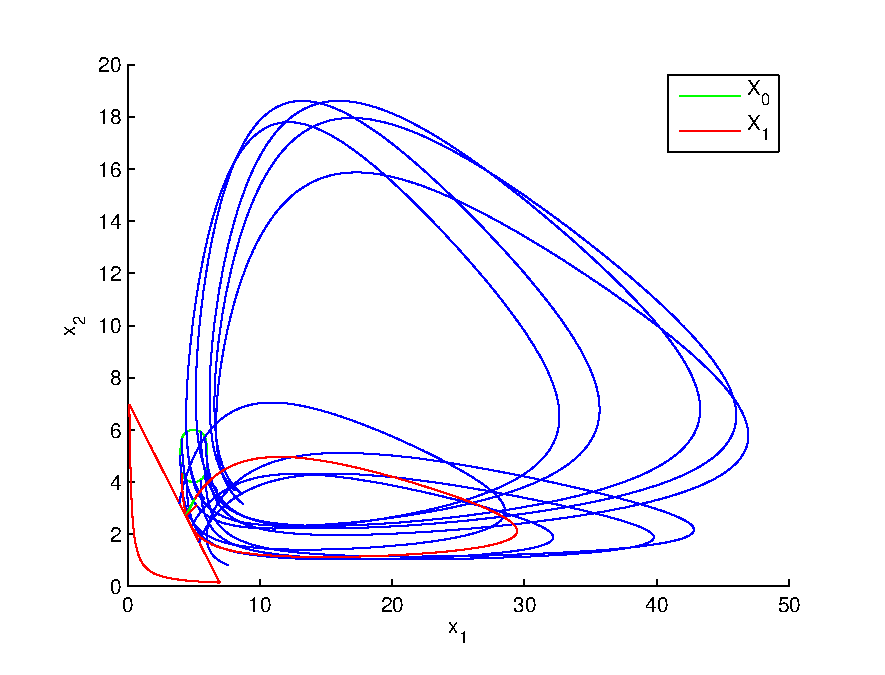
\includegraphics[scale=1]{pics/pic3_x_7.11.eps} \newline

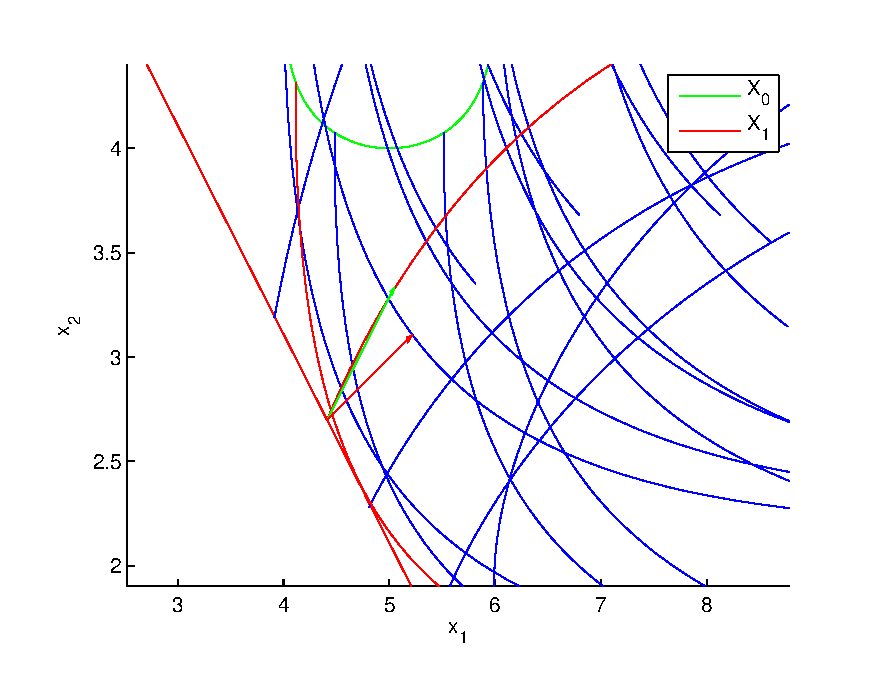
\includegraphics[scale=1]{pics/pic3_x_7.11_zoom.eps}

Результат: время 5.79. Но, изменив $a$ на 7.12, получим:

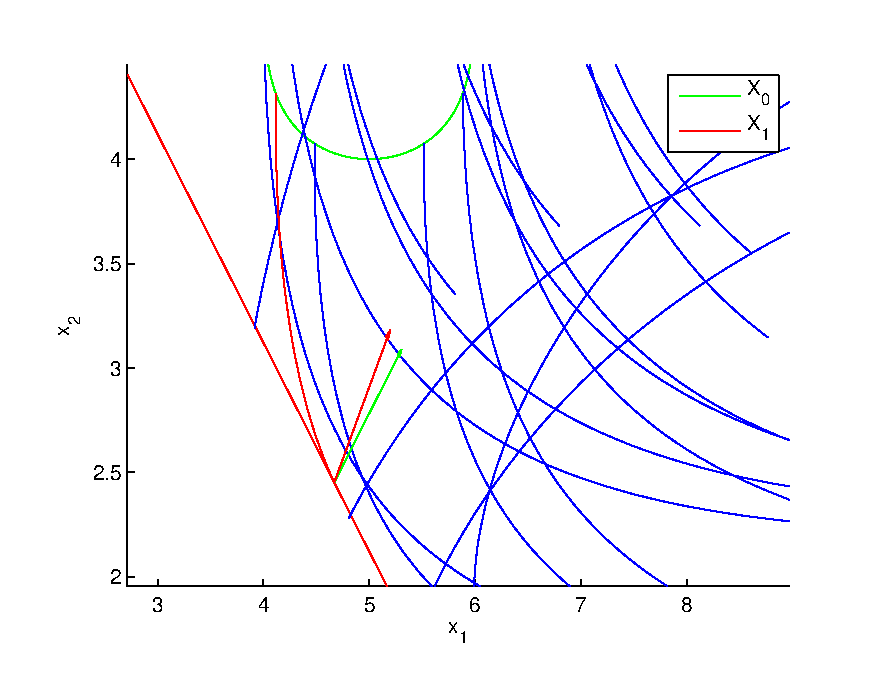
\includegraphics[scale=1]{pics/pic3_x_7.12.eps}

Время во втором случае 0.52. При просмотре графиков очевиден разрыв времени по конечному множеству. Он происходит из-за того, что фазовые траектории закручиваются, в некоторый момент удаляясь от целевого множества $\mathcal{X}_1$. Но при незначительном увеличении $a$ пересечение с траекториями происходит на предыдущем витке и с меньшим временем.
\pagebreak
\addcontentsline{toc}{section}{Список литературы}
\begin{thebibliography}{99}
	\bibitem{PBGM} Понтрягин~Л.~С., Болтянский~В.~Г., Гамкрелидзе~Р.~В., Мищенко~Е.~Ф. Математическая теория оптимальных процессов. М:~ Наука, 1976.
	\bibitem{Arutyunov} Арутюнов~А.~В., Магарил~--Ильяев~Г.~Г., Тихомиров~В.~М. Принцип максимума Понтрягина. М: Факториал Пресс, 2006.
\end{thebibliography}
\end{document}
